\documentclass[11pt, spanish]{article}
\usepackage[utf8]{inputenc}
\usepackage{listings} 
\usepackage{graphicx}
\usepackage{color,soul}
\usepackage[dvipsnames]{xcolor}
\usepackage[T1]{fontenc}
\usepackage{bigfoot}
\usepackage{amsmath}
\usepackage{commath}
\usepackage[numbered,framed]{matlab-prettifier}
\usepackage{caption}
\usepackage[figurename=Figura, tablename=Tabla, font={small,tt}]{caption}

\makeatletter
    \setlength\@fptop{0\p@}
\makeatother

\usepackage{geometry}
 \geometry{
 a4paper,
 left=30mm,
 right=30mm,
 top=30mm,
 }

\date{}

\lstset{
	style              = Matlab-editor,
  	basicstyle         = \mlttfamily,
  	escapechar         = ",
  	mlshowsectionrules = true,
	framesep=4.5mm,
	framexleftmargin=2.5mm,
	fillcolor=\color{White},
	rulecolor=\color{Black},
	numberstyle=\normalfont\tiny\color{Black}
}

\captionsetup[lstlisting]{font={small,tt}}
\renewcommand{\lstlistingname}{Script}



\begin{document}

\renewcommand\lstlistlistingname{Lista de Scripts}

\author{Sebastián Valencia Calderón \\ 201111578}
\title{Laboratorio 1: Sistema numérico de punto flotante}
\maketitle

%====================================================================
\section{Introducción}

La aritmética de punto flotante, proporciona las bases para la representación de cantidades reales en un computador digital. Dado que los cálculos numéricos son de fundamental importancia para el diseño de sistemas de ingeniería, y solución de grandes y complejos sistemas matemáticos, conviene entender los modos de representación de una cantidad real en un computador, y las implicaciones que esto tiene para los cálculos en cuestión. Las implicaciones, radican en la limitación básica del sistema; un computador digital, permite únicamente la representación de cierto conjunto de números con precisión finita. Esta limitación física para la representación de las cantidades, puede traer errores en los cálculos numéricos ejecutados por algoritmos implementados sobre un lenguaje de programación.\\

En este caso en particular, se estudia tal representación y sus limitaciones haciendo uso de \textsc{MATLAB}, una poderosa herramienta de computación científica, en la cual resulta pertinente la implementación de algoritmos numéricos, por su facilidad para representar y manipular arreglos de números. Mediante distintas aproximaciones, se pretende conocer las limitaciones de representación de la maquina o mejor, la arquitectura de la maquina sobre los números reales. A través de las implementaciones realizadas, se pretende cumplir con los siguientes objetivos:

\begin{itemize}
\item Entender las características, ventajas y desventajas asociadas con las unidades de punto flotante que permiten el desarrollo de la computación numérica.

\item Observar casos que ilustran las precauciones que deben ser tenidas en cuenta en sistemas intensivos en computación numérica.
\end{itemize}


%==================================================================
\section{Procedimiento}

Para cumplir los objetivos enumerados anteriormente, se desarrollan algoritmos para encontrar el epsilon ($\epsilon_M$) de la maquina de un número particular. Con base en esto, se comparan los algoritmos, y de manera análoga, los resultados para un rango grande de los números representados en la máquina donde los algoritmos fueron ejecutados. Después, se procede con la experimentación sobre el rango de números representables, y las cantidades matemáticas fundamentales en \textsc{MATLAB}, posteriormente, se estudian y desarrollan algoritmos numéricos que manipulan la representación de los números para obtener las representaciones numéricas de los resultados ya conocidos de manera analítica.

De manera más desglosada, la ejecución de este laboratorio, procede de la siguiente forma:

\begin{enumerate}

\item Implementar un algoritmo numérico que halle de manera eficiente y certera el epsilon de la maquina ($\epsilon_M$), esto es el valor que caracteriza el nivel de precisión de una máquina. El epsilon de la máquina, es el número de punto flotante más pequeño tal que: \cite{forsythe1977computer}

$$1 + \epsilon_M > 1$$

La definición dada anteriormente, es caracterizada únicamente por un número representado en punto flotante. Luego de esto, se pretende generalizar el epsilon sobre cualquier número, es decir, para un número $x$, $\epsilon(x) = \epsilon \ ;\ \abs{x + \epsilon} > x$. Con una distribución representativa de los números en punto flotante representables por la máquina de trabajo, se pretende comparar distintos algoritmos para su cálculo, y su valor en términos de $x$.

\item Con base en el estándar IEEE 754-2008 \cite{ieeestd}, se estudia la representación y de constantes matemáticas de importancia analítica, es decir, la representación numérica de algunos resultados analíticos fundamentales. De la misma manera, se calcula el valor de funciones matemáticas de interés y conocimiento general, esto, con el fin de dilucidar las implicaciones que pueda tener el desarrollo de modelos con base en cálculos numéricos sobre un computador digital.

\end{enumerate}

%==================================================================
\section{Resultados}

A continuación, se evidencian los resultados y la metodología y herramientas de ejecución para cada uno de los problemas propuestos en la guía de laboratorio.

\begin{enumerate}

\item "El valor epsilon de una maquina es la diferencia entre 1.0 y el numero de punto flotante siguiente. Ya que este espaciamiento no es uniforme en todo el rango de representación de números de punto flotante, esta definición puede ser extendida alrededor de cualquier otro numero (diferente de 1.0) y escrita como $\epsilon_M(x)$ para cualquier numero de punto flotante $x$. Esta es una de las razones para calcular el valor de epsilon en \textsc{MATLAB} (el cual cuenta por defecto con un valor constante “eps”), adicionalmente, es conveniente conocer algunos algoritmos para computar este valor, ya que algunos lenguajes de programación no cuentan un valor predefinido del mismo." (Tomado de la guía de laboratorio).\\

En el script \ref{lst:MaqEpsOne}, se evidencia el diseño y escritura de un algoritmo para calcular $\epsilon_M$. El script, muestra el algoritmo propuesto en el enunciado. Después de su ejecución, el valor fue:

$$\epsilon_M = 2.220446049250313 \times 10 ^{-16}$$

La constante eps de \textsc{MATLAB}, es: $2.220446049250313 \times 10^{-16}$.

\item Para generalizar la definición de $\epsilon_M$, sobre cualquier número, se introduce el concepto de $\epsilon_M(x)$, es decir, el número en punto flotante más pequeño para el cual resulta que sumarlo a $x$, se tiene un número mayo a $x$ en la representación del computador. Es decir, $\epsilon(x) = \epsilon \ ;\ \abs{x + \epsilon} > x$. Para diseñar un algoritmo que compute esto, resulta pertinente recurrir al script \ref{lst:MaqEpsOne}, en este, se cuenta con un valor de inicializacion de $\epsilon$, de manera que $1.0 + epsilon > 1.0$. Para la generalización requerida, se debe tener un $\epsilon$, tal que $x + \epsilon > x$, de manera que se doble el valor de $\epsilon$, y se incremente la suma $x + \epsilon$ hasta que $x + \epsilon \leq x$, se ha encontrado el valor $2 \times \epsilon$. En el script \ref{lst:MaqEps}, se evidencia el desarrollo de un algortimo, que análogamente al enunciado anteriormente, reduce el valor de $\epsilon$, hasta que $x + \epsilon \leq x$.

\lstinputlisting[caption = {Gráfica de $x$ vs $\epsilon(x)$. (plotEpsilon.m)}, label={lst:plotEpsilon}]{data/scripts/plotEpsilon.m}

\begin{figure}[htbp]
\centering
	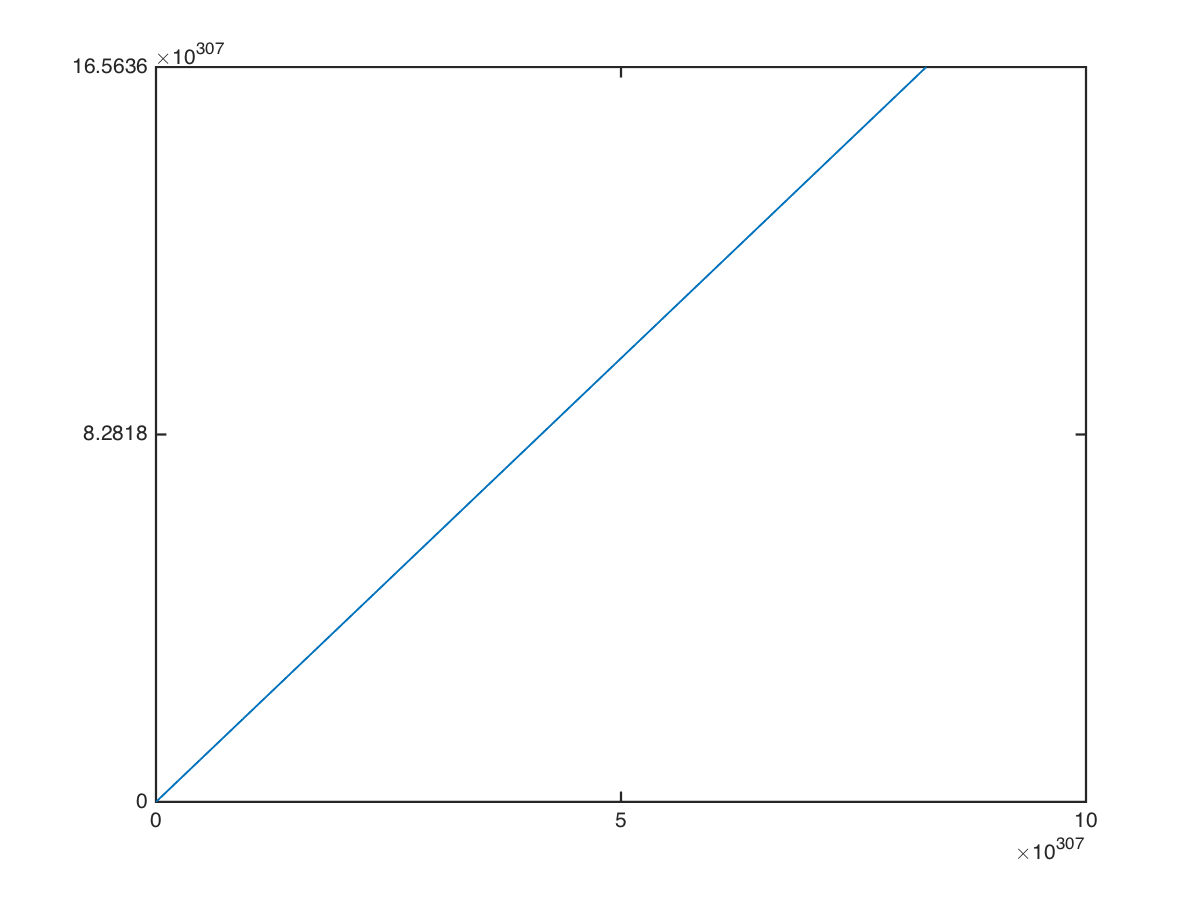
\includegraphics[scale=0.6]{data/img/plot_epsilon}
	\caption{Gráfica de $x$ vs $\epsilon_M(x)$}
\end{figure}

En la gráfica anterior, puede verse que entre más grande sea $x$, más grande es su epsilon definido como se definió anteriormente. El crecimiento de este patrón es lineal, lo cual es determinado por la representación de los números reales en un computador.

\item El procedimiento diseñado por William Kahan, y utilizado en el paquete \textsc{LINPACK}, implementado en \textsc{FORTRAN 77} \cite{dongarra1979linpack}, tiene como objetivo estimar las unidades de redondeo en una cantidad proporcional al tamaño de $x$. Es decir, el epsilon para un $x$ en punto flotante. Sin embargo, asume ciertas características, que son riesgosas si no se usa este de manera adecuada. Por ejemplo, la base usada para la representación en punto flotante no debe ser potencia de tres. El código original, puede verse en el script \ref{lst:kahanFortran}.\\

Para analizar el desempeño de este y comparar sus resultados con los implementados previamente, se procede a implementar el algoritmo en \textsc{MATLAB}, realizar pequeños experimentos para comparar los valores, y posteriormente, realizar la prueba sobre un rango representativo de los números de punto flotante capaces de ser representados por la máquina digital que corre los programas.

\begin{figure}[htbp]
\centering
	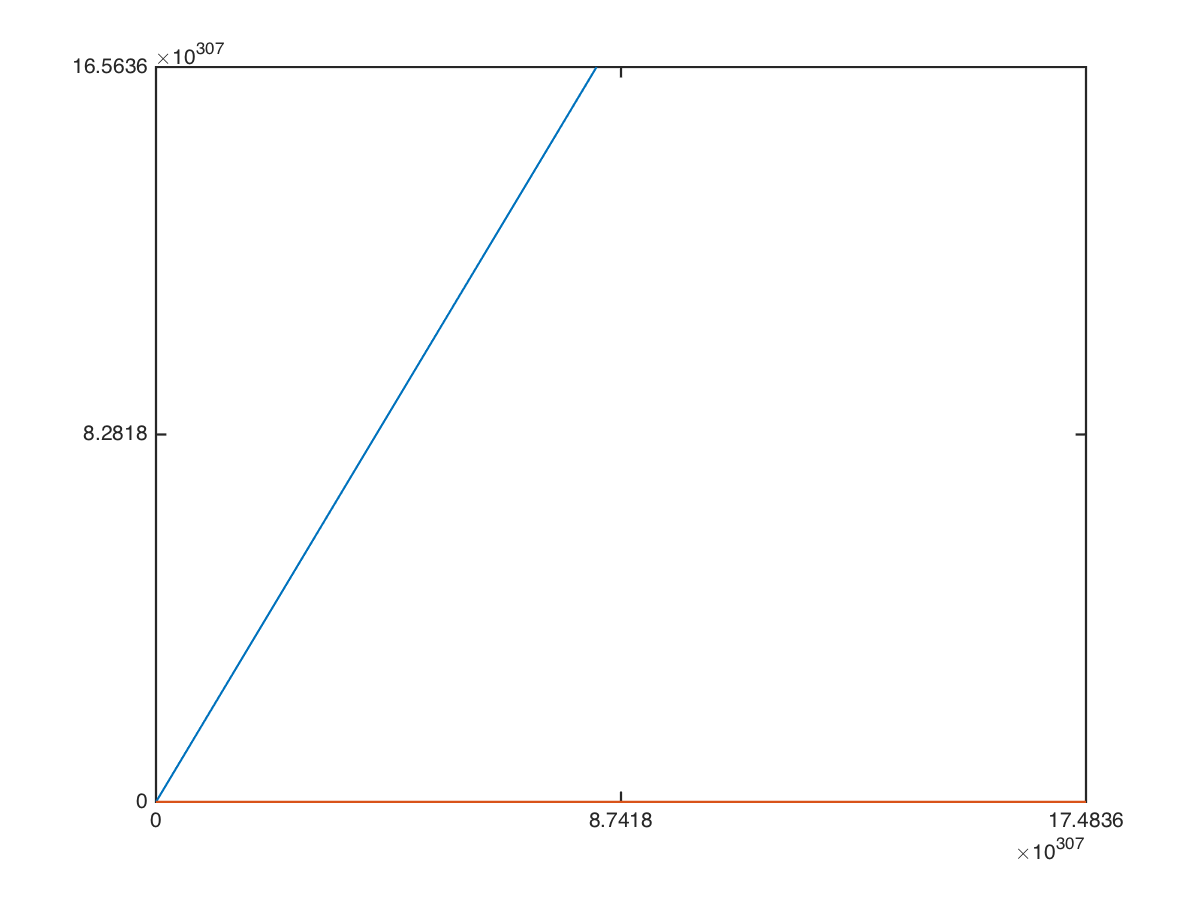
\includegraphics[scale=0.6]{data/img/plot_epsiloncomp}
	\caption{Gráfica de $x$ vs $\epsilon_M(x)$, los distintos trazos, muestran el epsilon de Kahan y el implementado anteriormente.}
\end{figure}

Puede verse en la gráfica anterior, que la precisión del algoritmo de Kahan, favorece la implementacion y análisis de resultados de los algoritmos numéricos desarrollados. Sin embargo, si estos resultados se cotejan con la arquitectura de la maquina, estos carecen de sentido. La diferencia en magnitud de ambos valores es demasiado grande, y se sabe que por la representación de los números dentro de un computador digital, a medida que va creciendo un numero, la diferencia entre el siguiente numero mas grande representado y el mismo va aumentando. Se determina que es mas confiable el algoritmo implementado. Además, no tiene restricciones. 

\item Después de investigar el estándar de la IEEE \cite{ieeestd}, para la representación y manipulación de los números reales en un computador digital, puede decirse de las siguientes constantes lo siguiente:

\begin{itemize}
\item $eps$. Su valor es 2.220446049250313e-16. Este valor, es la mínima distancia reconocida entre dos números de punto flotante $x$ y $y$. Es decir, la diferencia entre un numero $x$ en punto flotante según la representación definida por el estándar de la IEEE, y el siguiente numero que la maquina puede representar bajo el mismo estándar.

\item $realmax$. Su valor es 1.797693134862316e+308. Es el valor máximo representable en punto flotante según el estándar de la IEEE para la representación de los mismos.
\item $realmin$. Su valor es 2.225073858507201e-308. Es el valor mínimo representable en punto flotante según el estándar de la IEEE para la representación de los mismos. Claro está, sobre la máquina que corre el algoritmo.
\item $1/realmin$. Su valor es 4.494232837155790e+307. Representa valores anormales según la definición del estándar de la IEEE.
\item $1/realmax$. Su valor es 5.562684646268003e-309. Representa valores anormales según la definición del estándar de la IEEE.
\end{itemize}

\item A continuación, se brinda el valor de \textsc{MATLAB} para los valores indeterminados, y se brinda una posible explicación.

\begin{itemize}
\item $\frac{0}{0}$
\item $\frac{\infty}{\infty}$
\item $\infty * 0$
\item $1^{\infty}$
\item $\infty - \infty$
\item $0^\infty$
\item $\infty ^0$
\end{itemize}

Las operaciones listadas anteriormente, están definidas en el estándar de la IEEE \cite{ieeestd}. Los últimos dos, poseen un valor definid por el estándar siguiendo los preceptos básicos del análisis real: "todo número elevado a la cero es uno", "cero elevado a cualquier cosa es cero". Sin embargo, los demás se encuentran definidos en el estándar  haciendo uso de la constante NaN.\\

El símbolo NaN, denota Not a Number. Este símbolo, representa los valores que analíticamente o numéricmente no representa un número real. Su representación es a través de la cadena de bits con todos los exponentes en uno, y ceros en la mantisa. Los valores  $\frac{0}{0}$, $\frac{\infty}{\infty}$, $\infty * 0$, $1^{\infty}$, $\infty - \infty$, denotan en \textsc{MATLAB}, y en el estándar el valor NaN. \cite{ieeestd}, \cite{stallins}.

\item Dado que analíticamente $sin(\pi) = 0 \wedge cos(\pi) = -1 \wedge sin(\pi)^2 + cos(\pi)^2 = 1$, se investiga su valor en \textsc{MATLAB}, y se explica este valor.

\begin{itemize}
\item $sin(\pi)$. En \textsc{MATLAB}, su valor es 1.224646799147353e-16, esto se debe a la representción de $\pi$ en el computador, es decir, la forma de calcularlo (es necesario recordar que se trata de un valor irracional, y sus dígitos son infinitos.), y a la representación o algoritmo utilizado para encontrar $sin$, de un valor.
\item $cos(\pi)$. En \textsc{MATLAB}, su valor es -1, lo cua puede deberse a un cortocircuito en la implementación interna del algoritmo para encontrar $cos$ de un valor dado.
\item $sin(\pi)^2 + cos(\pi)^2$. En \textsc{MATLAB}, su valor es 1. Lo cual se debe a que se está sumando un valor cercano a cero con uno, y la diferencia entre estos dos valores es menor al epsilon de la máquina.
\end{itemize}

\item A continuación, se listan y explican los cálculos propuestos en el contexto del estándar IEEE 754-2008, \cite{ieeestd}.

\begin{itemize}
\item $(1 + 1E-16) - 1 \sim 0$
\item $(1 + 2E-16) - 1 \sim 2.2204E-16$
\item $(1 - 1E-16) - 1 \sim -1.1102E-16$
\item $1 + (1E-16 - 1) \sim 1.1102E-16$
\end{itemize}

\item Para encontrar el valor numérico de la expresión analítica definida como $\sum_{k=1}^{3000} \frac{1}{k^2} =  1.6446$, en \textsc{MATLAB} con cuatro cifras significativas, se presenta una alternativa. La alternativa propuesta en la guía, corta en cada paso el valor acumulado de la suma. El script propuesto, se muestra a continuación.

\lstinputlisting[caption = {Cálculo de $\sum_{k=1}^{3000} \frac{1}{k^2}$, usando redondeo en cada etapa intermedia. El resultado de ésta computación, varía mucho sobre el deseado. (badSummation.m)}, label={lst:badSummation}]{data/scripts/badSummation.m}

El valor resultante de este cálculo, es 1.6240, el cual está muy lejos del valor analítico deseado. Para esto, se propone la siguiente solución:

\lstinputlisting[caption = {Cálculo de $\sum_{k=1}^{3000} \frac{1}{k^2}$, usando redondeo en el resultado final. El resultado de ésta computación, es parecido al valor analítico del mismo. (summation.m)}, label={lst:summation}]{data/scripts/summation.m}

La cancelación en el script \ref{lst:badSummation}, se da por que es en cada etapa intermedia, interfiriendo los resultados del cálculo en cada iteración, es decir, el valor acumulado varía mucho en cada redondeo, pues se suma el valor actual con la nueva expresión para calcular el nuevo valor, pero se redondea la suma. De tal manera, el resultado nuevo ya está redondeado. En el procedimiento propuesto (script \ref{lst:summation}), se redondea el valor hasta lo ultimo, cuando ya todo el cálculo numérico, haya sido consumido por la iteración. El valor resultado del último método listado es: 1.6446.

\item La constante $e$, definida como $2.7182818$, es definida analíticamente como un límite al infinito de una expresión aritmética. Ésta expresión, sugiere una aproximación para su implementación por computador. Sin embargo, el planteamiento debe lo suficientemente bueno como para brindar eficiencia y precisión.  A continuación, se muestran la definición analítica, y la aproximación por computador.

$$e = \lim_{n\to\infty} \left( 1 + \frac{1}{n}\right)^n \Rightarrow e \sim \left( 1 + \frac{1}{n}\right)^n\ n\ \textsf{suficientemente grande}$$

Dada la anterior definición, se procede a diseñar un Script en \textsc{MATLAB} para encontrar un valor numérico a tal constante. El script \ref{lst:plotEpsilonComp}, muestra el algoritmo diseñado para encontrar de manera numérica e iterativa un valor aproximado de $e$. Este da pasos de 100, en 100 hasta que la diferencia entre el valor hallado y el real convenga con un nivel de tolerancia definido por la entrada de la función. Experimentado con esta función, se encuentra que para niveles de tolerancia significativamente grandes, se tiene que el valor hallado es muy lejano al real, sin embargo, con niveles de tolerancia entre 0.1 y 0.000001, el valor encontrado por el algoritmo es cercano al real. Mientras más el nivel de tolerancia se acerca a 0.000001, se tiene un valor más cercano al real. Al pasar este limite (0.000001), la precision requerida por el computador, no alcanza a cubrir los requerimientos de la maquina. En este ultimo caso, el valor resultado del cálculo es NaN. Sobre la eficiencia, puede verse que el algoritmo n itera sobre todos los números hasta alcanzar convergencia, sino da pasos de 100 en 100 hasta lograr esto.

\end{enumerate}

%==================================================================
\section{Conclusiones}

Por medio del desarrollo de los ejercicios numéricos propuestos, se determinó la importancia de contemplar la presencia del error en los cálculos que apoyan los modelos, diseños y simulaciones realizadas en ingeniería. Ya que el análisis numérico y la computación científica desempañan un papel muy importante en el desarrollo moderno de la ciencia y la ingeniería, es importante saber que las máquinas digitales que corren los algoritmos numéricos son maquinas de recursos limitados para la representación y manipulación de números reales y enteros; los cual tiene una importancia demasiado grande a la hora de solucionar problemas usando un computador. A manera de lista, se enuncian los principales hallazgos del desarrollo de la guía.

\begin{itemize}
  \item La presencia de errores numéricos, puede llevar a grandes problemas si estos no se contemplan en el diseño de una solución por computador. Es necesario tener cuidado al comparar expresiones analíticas con expresiones numéricas.
  
  \item La solución de sistemas numéricos por medio de computador, depende demasiado de la arquitectura y especificaciones técnicas de la máquina que corre los algoritmos. De la misma manera, el lenguaje de programación, la eficiencia y presicion de los algoritmos, son aspectos de fundamental importancia al evaluar una solución numérica y por computador de un problema.
  
  \item El estándar IEEE amplia-mente citado en el desarrollo de la, sienta una base solida para el desarrollo de la arquitectura de un computador y el tratamiento de los tipos de datos numéricos en un lenguaje de programación. Este busca ordenar y definir la representación de los números según la arquitectura de un computador y constituye una guía para los implementadores de las arquitecturas y los lenguajes de programación, las principales herramientas de trabajo de un analista. Es de fundamental importancia la existencia de estos estándares para minimizar la importancia de la maquina que corre los algoritmos.
   
\end{itemize}

%==================================================================
\newpage
\section{Bibliografía}

\begingroup
\renewcommand{\section}[2]{}%
\begin{thebibliography}{}

  \bibitem{forsythe1977computer} Forsythe, G.E. and Malcolm, M.A. and Moler, C.B. {\em Computer methods for mathematical computations}, Prentice-Hall series in automatic computation. 1977.
  
  \bibitem{ieeestd} IEEE Task P754. {\em IEEE 754-2008, Standard for Floating-Point Arithmetic}, pub-IEEE-STD. 2008.
  
  \bibitem{dongarra1979linpack} Dongarra, J.J. and Bunch, J.R. and Moler, C.B. and Stewart, G.W. {\em LINPACK Users' Guide}, Society for Industrial and Applied Mathematics. 1979.
  
  \bibitem{stallins} Stallins, W. {\em Computer Organization and Architecture}, Pearson Education. 2013.
  
\end{thebibliography}
\endgroup

%==================================================================
\newpage
\section{Scripts}

\lstinputlisting[caption = {Cálculo de $\epsilon_M$. (MaqEpsOne.m)}, label={lst:MaqEpsOne}]{data/scripts/MaqEpsOne.m}

\lstinputlisting[caption = {Cálculo de $\epsilon_M$ para un $x$ específico. (MaqEps.m)}, label={lst:MaqEps}]{data/scripts/MaqEps.m}

\lstinputlisting[caption = {Cálculo de $\epsilon_M(x)$ según el algoritmo de Kahan implementado en \textsc{FORTRAN}. (kahan.f)}, label={lst:kahanFortran}, language=Fortran]{data/scripts/kahan.f}

\lstinputlisting[caption = {Cálculo de $\epsilon_M$ para un $x$ específico. (KahanEpsilon.m)}, label={lst:kahanMatlab}]{data/scripts/KahanEpsilon.m}

\lstinputlisting[caption = {Cálculo de $\epsilon_M$ para un $x$ específico. (plotEpsilonComp.m)}, label={lst:plotEpsilonComp}]{data/scripts/plotEpsilonComp.m}

\lstinputlisting[caption = {Función en \textsc{MATLAB} para encontrar de manera numérica el valor de $e$ con cierta tolerancia o diferencia absoluta con el valor real (el definido en \textsc{MATLAB}). (FindExp.m)}, label={lst:plotEpsilonComp}]{data/scripts/FindExp.m}

\addcontentsline{toc}{chapter}{\lstlistlistingname}
\lstlistoflistings

\bibliography{sample}

\end{document}
